% !TeX spellcheck = en_US

\chapter{Generating Minimal DFAs} \label{ch:3}

We seek algorithms for generation of minimal DFAs that fulfill the conditions defined in the requirements analysis section~\ref{ch:2:requirements-analysis}. We formally subsume these conditions via the GenerateNewMinimalDFA-problem:
\begin{definition}[GenNewMinDFA] $ $ \\
	$ $ \vspace{-0.4cm} \\
	\noindent $\underline{\emph{Given:}}$
	\vspace{-0.5cm}
	\begin{align*}
	\nSO \in \mathbb{N}\ \ \ & \emph{number of states} \\
	\kAL \in \mathbb{N}\ \ \ & \emph{alphabet size} \\
	\nF \in \mathbb{N}\ \ \ & \emph{number of final states} \\
	d \in \mathbb{N}\ \ \ & \emph{value of $\mmD(A_{sol})$} \\
	p \in \{0,1\}\ \ \ & \emph{planarity-bit}
	\end{align*}
	\noindent $\underline{\emph{Task:}}$ \emph{Compute, if it exists, a solution DFA $A_{sol}$ with}
	\begin{itemize}
		\item $|Q_{sol}|=\nSO$, $|\Sigma_{sol}|=\kAL$, $|F_{sol}|=\nF$
		\item $d = \mmD(A_{sol})$
		\item $A_{sol}$ \emph{being planar iff} $p = 1$
		\item $L(A_{sol})$ \emph{being new}
	\end{itemize}
\end{definition}
\noindent To solve this problem we present one approach in much detail. Afterwards an alternative approach and related work will be discussed.

\begin{remark}\label{ch:3:rem:qas-set}
	For all generated DFAs we are going to set $Q_{sol} = [[\nSO]] = \{0,\ldots,\nSO-1\}$, $\Sigma_{sol} = [[\kAL]] = \{0,\ldots,\kAL-1\}$ and $s_{sol} = 0$, so every DFA of same state number and alphabet size will have the same states and symbols.
\end{remark}
\noindent As a consequence the presented algorithms will not be able to compute all of $\Amin$.

\section{Using a Rejection Algorithm}

We describe a procedure that is essentially a \emph{rejection algorithm} adjusted to find DFAs with the properties determined by the input parameters. The approach works as follows:

Firstly a \emph{test} DFA $A_{test}$ is generated by use of either randomness or enumeration. Alphabet size and number of (final) states will already be correct. On this DFA then tests will be executed, to check if it is minimal, planar (if wished) and has not been generated before. If this is the case, $A_{test}$ will be returned, if not, new test DFAs are generated until all tests pass.

A note on the search space. If we would not restrict ourselves to $Q_{sol} = [[\nSO]]$ and $\Sigma_{sol} = [[\kAL]]$, then for a given number of states $\nSO$ and symbols $k$, the number of possible state sets and alphabets would be infinite. This way however we do not have to iterate through infinitely many same-sized versions of $Q_{sol}$ respectively $\Sigma_{sol}$. Since there is a finite number of possible transitions functions and final state sets given $\nSO, \kAL$, we can now even guarantee that the enumerating variant of our algorithm is going to terminate.

Here follows a description of our general algorithm for generating minimal DFAs.
\vspace{0.2cm}
\begin{algorithmic}[1]
	\Function{GenNewMinDFA-1\ }{$\nSO, \kAL, \nF, d \in \mathbb{N}, p \in \{0,1\}$}
		\While {True}
		
			\vspace{0.2cm}
		
			\State generate DFA $A_{test}$ with $|Q|, |\Sigma|, |F|$ matching $\nSO, \kAL, \nF$
			
			\vspace{0.2cm}
			
			\If {$A_{test}$ not minimal \textbf{or not} $\mmD_{min} \leq \mmD(A_{test}) \leq \mmD_{max}$}
				\State \textbf{continue}
			\EndIf
			
			\If {$p = 1$ \textbf{and} $A_{test}$ is not planar}
				\State \textbf{continue}
			\EndIf
			
			\If {$L(A_{test})$ is not new}
				\State \textbf{continue}
			\EndIf
			
			\vspace{0.2cm}
			
			\State\Return $A_{test}$
		\EndWhile
	\EndFunction
\end{algorithmic}
\vspace{0.2cm}
We will complete \textsc{GenNewMinDFA} by resolving how the tests in lines $4, 6$ and $8$ work and by showing two methods for generation of DFAs with given restrictions of $|Q|, |\Sigma|$ and $|F|$.

\subsection{Ensuring D-value lies in range and Minimality}

In order to test, whether $A_{test}$ is minimal, it is sufficient to ensure, that $A_{test}$ has no equivalent state pairs and no unreachable states.

To get $\mmD(A_{test})$, we have to run \CompDist\ (or a variant) entirely. Hence we can combine the test for the existence of equivalent state pairs with computing the DFAs $\mmD$-value:
\vspace{0.2cm}
\begin{algorithmic}[1]
	\Function{HasEquivalentStates}{$A$}
		\State $depth \gets 0$ \Comment{will be $\mmD(A)$ in the end}
		\State $M \gets \{ (p,q), (q,p)\ |\ p \in F, q \notin F \}$
		\Do
			\State $depth \gets depth + 1$
			\State $M' \gets \{ (p,q)\ |\ (p,q) \notin M \land \exists \sigma \in \Sigma \colon (\delta(p,\sigma), \delta(q,\sigma)) \in M \}$
			\State $M \gets M \cup M'$
		\doWhile {$M' \neq \emptyset$}
		\State $hasDupl \gets | \{ (p,q)\ |\ p \neq q \land (p,q) \notin M \} | > 0$
		\State \Return $hasDupl, depth$
	\EndFunction
\end{algorithmic}
\vspace{0.2cm}
Since \CompDist\ basically computes all distinguishable state pairs $\not\sim_A$, we test in line $9$, whether there is a pair of distinguishable states not in $\not\sim_A$.

Regarding the unreachable states, we can just use \CompUnr\ and test whether the computed set is empty:
\vspace{0.2cm}
\begin{algorithmic}[1]
	\Function{HasUnreachableStates}{$A$}
	\State \Return $|\CompUnr(A)| > 0$
	\EndFunction
\end{algorithmic}

\subsection{Ensuring Planarity}\label{ch:3:sec:planarity}

There exist several algorithms for planarity testing of graphs. In this work, the library \emph{pygraph}\footnote{\url{https://github.com/jciskey/pygraph}} has been used, which implements the Hopcroft-Tarjan planarity algorithm. More information on this can be found for example in this~\cite{Koc93} introduction from William Kocay. The original paper describing the algorithm is by Hopcroft and Tarjan~\cite{HT74}.

\subsection{Ensuring Uniqueness}

In our requirements we stated, that we wanted the generated solution DFA to be new, meaning it should have a unique language compared to all previously generated solution DFAs. This implies the need of a database, such that we can save and load the list $l$ of already found DFAs. We name this database $\text{DB}_\text{found}$.

In DB$_{found}$ only minimal DFAs will be saved, since every solution DFA is minimal. Furthermore every test DFA $A_{test}$ is guaranteed to be minimal, since non-minimal test DFAs are filtered out beforehand.

Theorem~\ref{ch:2:thm:uniq-ism} states that two minimal DFAs have the same language, iff they are isomorph. So we can use an isomorphism test to decide whether two DFAs have the same language.

However this test can be constructed more efficient: Two minimal DFAs cannot be isomorph, if their number of states, alphabet size or number of final states differ. It would thus suffice to compare the test DFA only against those DFAs from the database that match the parameters $\nSO, k, \nF$. As a consequence we propose the following scheme for DB$_{found}$, which is assumed to be a relational database:
\begin{center}
	\begin{tabular}{c c c c c c}
	$|Q_A|$ & |$\Sigma_A$| & $|F_A|$ & $\mmD(A)$ & $isPlanar(A)$ & $encode(A)$
	\end{tabular}
\end{center}
Now we need not fetch all DFAs every time but can select only the relevant ones.

A more concrete specification of the above discussed proceeding is shown below, embedded in the main algorithm:
\vspace{0.2cm}
\begin{algorithmic}[1]
	\Function{GenNewMinDFA-2\ }{$\nSO, \kAL, \nF, d, p$}
	
		\vspace{0.2cm}
	
		\State $l \gets$ all DFAs in DB$_{found}$ matching $\nSO, \kAL, \nF$
		
		\vspace{0.2cm}
		
		\While {True}
		
		\vspace{0.2cm}
		
			\State $\ldots$
			\If {$A_{test}$ is isomorph to any DFA in $l$}
				\State \textbf{continue}
			\EndIf
			
			\vspace{0.2cm}
			
			\State save $A_{test}$ and its respective properties in DB$_{found}$
			\State\Return $A_{test}$
		\EndWhile
	\EndFunction
\end{algorithmic}
\vspace{0.2cm}
A sample isomorphism test is described in Appendix~\ref{ch:app:ism-test}.

\subsection{Option 1: Generating Test DFAs via Randomness}

We now approach the task of generating a random DFA where alphabet and number of (final) states are set. For our generated DFA we choose $Q_{sol}$, $\Sigma_{sol}$ and the start state as explained in Remark~\ref{ch:3:rem:qas-set}.

The remaining elements that need to be defined are $\delta$ and $F$. The set of final states is supposed to have a size of $\nF$ and be a subset of $Q$. Therefore we can simply choose randomly $\nF$ distinct states from $Q$.

\noindent The transition function has to make the DFA complete, so we have to choose an ``end'' state $q'$ for every state-symbol-pair $q,\sigma$ in $Q \times \Sigma$. There is no restriction concerning $q'$, so we can randomly choose $\delta(q, \sigma) = q'$ from $Q$.

With defining how to compute $\delta$ we have covered all elements of a DFA.

\vspace{0.2cm}
\begin{algorithmic}[1]
	\Function{GenNewMinDFA-3a\ }{$\nSO, \kAL, \nF, d, p$}
	
		\vspace{0.2cm}
	
		\State $l \gets$ all DFAs in DB1 matching $\nSO, \kAL, \nF$
		\State $Q \gets[[\nSO]]$
		\State $\Sigma \gets [[\kAL]]$
		
		\vspace{0.2cm}
		
		\While {True}
		
		\vspace{0.2cm}
		
			\State $\delta \gets \emptyset$
			\For {$(q,\sigma)$ \textbf{in} $Q\times\Sigma$}
				\State $\delta(q,\sigma) = $ random chosen state from $Q$
			\EndFor
			\State $s \gets 0$
			\State $F \gets$ random sample of $\nF$ states from $Q$
			\State $A_{test} \gets (Q, \Sigma, \delta, s, F)$
			
			\vspace{0.2cm}
			
			\If {$A_{test}$ not minimal \textbf{or} $d \neq \mmD(A_{test})$}
			\State \textbf{continue}
			\EndIf
			
			\If {$p = 1$ \textbf{and} $A_{test}$ is not planar}
			\State \textbf{continue}
			\EndIf
			
			\If {$A_{test}$ is isomorph to any DFA in $l$}
			\State \textbf{continue}
			\EndIf
			
			\vspace{0.2cm}
			
			\State save $A_{test}$ and its respective properties in DB1
			\State\Return $A_{test}$
		\EndWhile
	\EndFunction
\end{algorithmic}
\vspace{0.2cm}

\subsection{Option 2: Generating Test DFAs via Enumeration}

% enumerating instead of random

The second method of test DFA generation is based on the idea, that instead of randomly generating $F$ and $\delta$, we could enumerate through all possible final state sets and transition functions. We will use the given parameters $\nSO, k, \nF$ to split up the enumeration space --- every enumeration yields only DFAs with the same $\nSO, k, \nF$.

% enumeration states

An enumeration is represented by an \emph{enumeration state} $s_{\nSO, k, \nF} = (F_F,F_\delta)$ consisting of two arrays\footnotemark. The first array shall have $\nSO$ Bits, where Bit $F_F[i] \in \{0,1\}$ represents the information, whether $i$ is a final state or not. The second array shall have $\nSO\kAL$ entries containing state names, such that entry $F_\delta[i * \kAL + j] = q, q\in [[\nSO]]$ says, that $\delta(i, j) = q$.

\footnotetext{We denote the two arrays (or \emph{fields}) as $F_F,F_\delta$ instead of $A_F,A_\delta$ to avoid confusion with the notation of DFAs.}

% -- EX example of the two fields and their meaning

\begin{example}
	{\raggedright\itshape Given $\nSO = 4$, $\kAL = 2$, $\nF = 3$. Note that for the sake of readability we will use $a,b,\ldots$ instead of $0,1,2,\ldots$ as alphabet symbols. An example $F_F$-array could be $1101$. Since $F_F[i]$ is $1$ for $i = 0,1,3$ the final states are:
	\begin{tabbing}
		\qquad$F = \{\ 0, 1, 3\ \}$
	\end{tabbing}
	{\raggedright A possible $F_\delta$-array could be $12013201$. The following table depicts, how $F_\delta$ assigns one state to every combination of states and symbols $(q,\sigma) \in Q\times\Sigma$ and thus defines $\delta$:\par}
	\begin{minipage}{.4\textwidth}
		\vspace{0.3cm}
		\begin{tabbing}
			\hspace{0.3cm}
			\begin{tabular}{r c;{3pt/1pt}c | c;{3pt/1pt}c | c;{3pt/1pt}c | c;{3pt/1pt}c }
				$q \in Q$\hspace{0.2cm} & \multicolumn{2}{c|}{$0$} & \multicolumn{2}{|c|}{$1$} & \multicolumn{2}{|c|}{$2$} & \multicolumn{2}{|c}{$3$} \\%\cline{2-9}
				
				$\sigma \in \Sigma$\hspace{0.2cm} & $a$ & $b$ & $a$ & $b$ & $a$ & $b$ & $a$ & $b$ \\\cline{2-9}
				
				%				State $p$ & $2$ & $3$ & $1$ & $2$ & $4$ & $3$ & $1$ & $2$
				
				$\delta(q,\sigma)$\hspace{0.2cm} & \multicolumn{1}{c}{$1$} & \multicolumn{1}{c}{$2$} & \multicolumn{1}{c}{$0$} & \multicolumn{1}{c}{$1$} & \multicolumn{1}{c}{$3$} & \multicolumn{1}{c}{$2$} & \multicolumn{1}{c}{$0$} & \multicolumn{1}{c}{$1$}
			\end{tabular}
		\end{tabbing}
		\vspace{0.01cm}
	\end{minipage}\hspace{1cm}
	\begin{minipage}{.4\textwidth}
		$\delta(0, a) = 1$, $\delta(0,b) = 2$,\\$\delta(1, a) = 0, \ldots$
	\end{minipage}\\}
	{\raggedright The corresponding DFA might look like this:}
	\begin{tabbing}
		\qquad\resizebox{.25\linewidth}{!}{
		\begin{tikzpicture}[initial text={},scale=1., every node/.style={transform shape}]
		\tikzstyle{every state}=[minimum size=5mm, inner sep=0pt]
		
		\node[initial, state,accepting] (0) at (0, 0)    {$0$};
		\node[state,accepting] 		    (1) at (2,0)     {$1$};
		\node[state] 					(2) at (0,-1.5)  {$2$};
		\node[state,accepting]          (3) at (2, -1.5) {$3$};
		
		\path[->]
		(0) edge [bend left]  node [above=-0.07cm] 		 {$a$} (1)
		(0) edge 			  node [left=-0.07cm]  		 {$b$} (2)
		(1) edge 			  node [above=-0.07cm]       {$a$} (0)
		(1) edge [loop above] node [right]        		 {$b$} (1)
		(2) edge 			  node [above=-0.07cm]		 {$a$} (3)
		(2) edge [loop below] node [left]  				 {$b$} (2)
		(3) edge 			  node [above right=-0.13cm] {$a$} (0)
		(3) edge 			  node [right=-0.07cm] 		 {$b$} (1)
		;
		\end{tikzpicture}
	}\end{tabbing}\vspace{-0.5cm}\hfill$\square$
\end{example}
% how to compute next DFA

\noindent Given an enumeration state $s_{\nSO, \kAL, \nF} = (F_F, F_\delta)$ we will then compute the next DFA based on this state as described in the following algorithm. We assume, that adding $1$ to a $n$-ary number $n-1\ n-1\ \ldots n-1$ yields $00\ldots0$.
\vspace{0.2cm}
\begin{algorithmic}[1]
	\Function{IncrementEnumProgress\ }{$F_F, F_\delta, \nSO, \kAL, \nF$}
	\State add $1$ to $(F_\delta)_\nSO$
	\If {$F_\delta = 0 \ldots 0$}
		\If {$F_F = 1\ldots10\ldots0$ \textbf{and} $\#_1(F_F) = \nF$}
			\State \Return $\bot$
		\EndIf
		\While {$\#_1(F_F) \neq \nF$}
			\State add $1$ to $(F_F)_2$
		\EndWhile
	\EndIf
	\State \Return $F_F, F_\delta$
	\EndFunction
\end{algorithmic}
\vspace{0.2cm} We will treat both fields as numbers, $F_F$ as $2$-ary and $F_\delta$ as $\nSO$-ary. To get to the next DFA, we will first increment $F_\delta$ by $1$. If all transitions functions have been enumerated ($F_\delta$ becomes $0\ldots0$), then we increment $F_F$ until it contains $\nF$ $1$'s (again) and enumerate all transition functions again.

Concerning the terminating behavior of \textsc{IncrementEnumProgress} consider the following observation:

% finite enumerations, how many

\begin{observation}
	An enumeration of DFAs given $\nSO, k, \nF$ will eventually terminate. Having a requirement of $\nF$ final states, then $\binom{\nSO}{\nF}$ is the number of possible $F$-configurations. On the other hand there are $\nSO^{\nSO\kAL}$ possible $\delta$-configurations: We have to choose one of $\nSO$ possible end states for every combination in $Q\times\Sigma$ - so $\nSO\kAL$ times.
\end{observation}

\noindent This leads us to the range of an enumeration which can be expressed using the first and last enumeration state:
\begin{itemize}
	\item $s_{\nSO, \kAL, \nF} = (F_F, F_\delta) = (0\ldots0\underbrace{1\ldots 1}_{\nF\ 1's},\ 0\ldots0)$
	\item $s_{\nSO, \kAL, \nF} = (F_F, F_\delta) = (\underbrace{1\ldots 1}_{\nF\ 1's}0\ldots0,\ \nSO-1 \ldots \nSO-1)$
\end{itemize}
Consequently the algorithm can terminate in two ways. Either a next DFA could be enumerated or all DFAs with $|Q|=\nSO, |\Sigma|=k, |F|=\nF$ have been found.

%As a consequence we will create enumeration states $F_F,F_\delta$ to concrete values of $\nSO, k, \nF$ only if DFAs of that kind are requested.

%The algorithm may terminate in two ways. Either $F_F, F_\delta$ have been successfully incremented, then line 9 is reached. Or $F_F = 1\ldots 1$ and $F_\delta = \nSO-1 \ldots \nSO-1$. Then $F_\delta$ becomes $0\ldots 0$ after incrementing and $F_F$ does not reach a state with $\nF$ $1$'s again through increment --- in this case all DFAs with $|Q|=\nSO, |\Sigma|=k, |F|=\nF$ have been enumerated.

% EX -- example of an enumProgress increment
	
\begin{example}
	We showcase a sample enumeration at points, that demonstrate the semantics of different increments. We will use $\nSO=4$, $\kAL=2$ and $\nF=2$. Note that we will use $a,b,\ldots$ instead of $0,1,\ldots$ as symbols. Valid enumeration progresses are depicted green.\par
	\vspace{0.4cm}\noindent
	\begin{minipage}{0.56\textwidth}
		We will start with the initial enumeration progress (1). In this case, a simple addition of $1$ to $F_\delta$ does not cause an overflow of $F_\delta$ (2), meaning the enumeration increment is already finished.\newline
		
		(3). In this state however $F_\delta$ becomes $0\ldots0$ (4) after adding $1$. Thus we add $1$ to $F_F$, until it contains the required number of ones again (so we always have $f$ final states). The next $4$-ary number with $2$ ones after $0011$ is $0101$ (5).\newline
		
		(6). Here $F_\delta$ is at its maximum and there is no higher $4$-ary number with $2$ ones. Thus the next enumeration step yields the state (7), that marks the enumeration end.
	\end{minipage}
	\hfill
	\begin{minipage}{0.4\textwidth}
		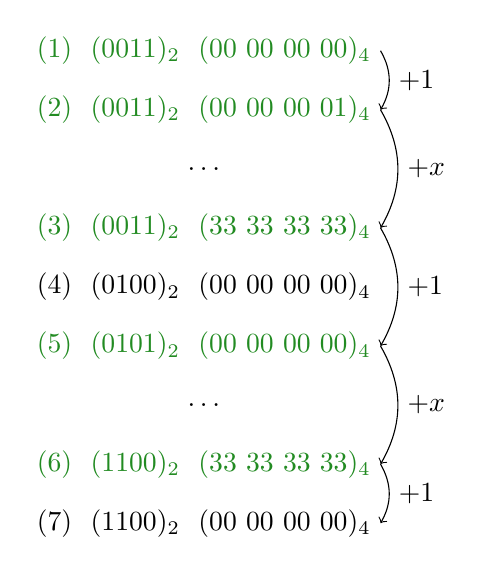
\begin{tikzpicture}
		\node (0) at (0,0) {\color{ForestGreen} (1)\ \ $(0011)_2\ \ (00\ 00\ 00\ 00)_4$} ;
		\node (1) at (0,-0.75) {\color{ForestGreen} (2)\ \ $(0011)_2\ \ (00\ 00\ 00\ 01)_4$} ;
		\node (2) at (0,-1.5) {$\ldots$} ;
		\node (3) at (0,-2.25) {\color{ForestGreen} (3)\ \ $(0011)_2\ \ (33\ 33\ 33\ 33)_4$} ;
		\node (4) at (0,-3) {(4)\ \ $(0100)_2\ \ (00\ 00\ 00\ 00)_4$} ;
		\node (5) at (0,-3.75) {\color{ForestGreen} (5)\ \ $(0101)_2\ \ (00\ 00\ 00\ 00)_4$} ;
		\node (6) at (0,-4.5) {$\ldots$} ;
		\node (7) at (0,-5.25) {\color{ForestGreen} (6)\ \ $(1100)_2\ \ (33\ 33\ 33\ 33)_4$} ;
		\node (8) at (0,-6) {(7)\ \ $(1100)_2\ \ (00\ 00\ 00\ 00)_4$};
		
		\path[->]
		(0.east) edge [bend left] node [right] {$+1$} (1.east)
		(1.east) edge [bend left] node [right] {$+x$} (3.east)
		(3.east) edge [bend left] node [right] {$+1$} (5.east)
		(5.east) edge [bend left] node [right] {$+x$} (7.east)
		(7.east) edge [bend left] node [right] {$+1$} (8.east)
		;
		\end{tikzpicture}
	\end{minipage}\par
	\hfill$\square$
\end{example}

\noindent Based on the incremented bit-fields the new DFA can be build according to the semantics defined above:
\vspace{0.2cm}
\begin{algorithmic}[1]
	\Function{DFAfromEnumProgress\ }{$F_F, F_\delta, \nSO, \kAL, \nF$}
	\State $Q \gets [[\nSO]]$
	\State $\Sigma \gets [[\kAL]]$
	\State $\delta \gets \emptyset$
	\For {$i$ \textbf{in} $[[\nSO]]$}
		\For {$j$ \textbf{in} $[[\kAL]]$}
            \State $\delta(i, j) = F_\delta[i * \kAL + j]$
		\EndFor
	\EndFor
	\State $s \gets 0$
	\For {$i$ \textbf{in} $[[\nSO]]$}
		\If {$F_F[i] = 1$}
			\State Add $i$ to $F$
		\EndIf
	\EndFor
	\State \Return $(Q, \Sigma, \delta, s, F)$
	\EndFunction
\end{algorithmic}
\vspace{0.2cm}

% saving enumProgress for later progression

\noindent Since it is not sensible to create initial enumeration states for all possible enumeration (there are infinite many, due to $\nSO\in\mathbb{N}$) we will create states by demand.

Once the enumeration to the next DFA within a call of \textsc{GenNewMinimalDFA} has been finished, it is reasonable to save the enumeration state, such that during the next call enumeration can be resumed from that point on. Thus we introduce a second database DB$_{states}$ with the following table:
\begin{center}
	\begin{tabular}{c c c c c c}
		$|Q_A|$ & |$\Sigma_A$| & $F_F$ & $F_\delta$
	\end{tabular}
\end{center}
In the following variant of \textsc{GenNewMinimalDFA} it can be seen how the enumeration method is integrated:
\vspace{0.2cm}
\begin{algorithmic}[1]
	\Function{GenNewMinDFA-3b\ }{$\nSO, \kAL, \nF, d, p$}
	
		\vspace{0.2cm}
	
		\State $l \gets$ all DFAs in DB$_{found}$ matching $\nSO, \kAL, \nF, d, p$
		
		\vspace{0.2cm}
		
		\If {$\exists$ enum.\ state for $\nSO, \kAL, \nF$ in DB$_{states}$}
			\State $F_F, F_\delta \gets$ load $s_{\nSO, \kAL, \nF}$ from DB$_{states}$
		\Else
			\State $F_F,F_\delta \gets 0\ldots0\underbrace{1\ldots1}_{\nF\ 1's}, 0\ldots0$
		\EndIf
		
		\vspace{-0.2cm}
		\newpage
		\While {True}
		
			\vspace{0.2cm}
		
			\If {$F_F, F_\delta$ is finished}
				\State save $F_F, F_\delta$
				\State\Return $\bot$
			\EndIf
			\State $A_{test} \gets$ next DFA based on $F_F, F_\delta$
			
			\vspace{0.2cm}
			
			\If {$A_{test}$ not minimal \textbf{or} $d \neq \mmD(A_{test})$}
				\State \textbf{continue}
			\EndIf
			
			\If {$p = 1$ \textbf{and} $A_{test}$ is not planar}
				\State \textbf{continue}
			\EndIf
			
			\If {$A_{test}$ is isomorph to any DFA in $l$}
				\State \textbf{continue}
			\EndIf
			
			\vspace{0.2cm}
			
			\State save $F_F, F_\delta$ in DB$_{states}$
			\State save $A_{test}$ and its respective properties in DB$_{found}$
			\State\Return $A_{test}$
		\EndWhile
	\EndFunction
\end{algorithmic}
\vspace{0.2cm}

\section{Related Work on DFA Generation}

Nicaud provides an overview of results on random generation and combinatorial properties of DFAs in ~\cite{Nic14}. We will outline relevant related work.

Nicaud's summary indicates, that research has focused on randomized generation of accessible, but not minimal DFAs so far. In the following we will sketch some approaches that have come up.

\paragraph*{Using the Recursive Method.}

Champarnaud and Paranthoën~\cite{CP05} continue ideas started by Nicaud in his thesis~\cite{Nic00}. Let $\mathfrak{F_{n,m}}$ be the set of extended $m$-ary trees of order $n$. These trees are characterized by a partitioning $V = N \uplus L$ with $|N| = n$ and the properties $v \in N \Rightarrow d^+(v) = m$ and $v \in L \Rightarrow d^+(v) = 0$. We define the following set of tuples using $s=n(m-1)$:
\[
    \mathfrak{R_{m,n}} = \{\ (k_1,\ldots,k_s) \in \mathbb{N}^s\ |\ \forall i\in [2,s]\colon k_i \geq \left\lceil\frac{i}{m-1}\right\rceil\ and\ k_i \geq k_{i-1}\ \}
\]
In~\cite[p. 6]{CP05} it is shown that there exists a bijection $\varphi$ between $\mathfrak{F_{n,m}}$ and $\mathfrak{R_{m,n}}$ which maps to $k_i$, $i\in[1,s]$ of a tuple the number of leaves visited before the $i$th leaf in a tree. The connection to accessible DFAs is established by proving that  ``transition structures\footnotemark''\ with $|Q|=n$, $|\Sigma|=m$ reduced to the set of the smallest paths from the $s$ to each other state are in bijection with extended $m$-ary trees of order $n$ (see~\cite[p. 8]{CP05}).

As a consequence Champarnaud and Paranthoën are able to construct a random generator of accessible complete DFAs using the ``recursive method'' from~\cite{NW78} which generates $n$-tuples~\cite[p. 10]{CP05}. Nicaud states in his survey that the algorithm's runtime is $\mathcal{O}(n^2)$ but notes, that generation of DFAs with more than ``a few thousand states'' is practically hard to do~\cite[pp. 10-11]{Nic14}.
\footnotetext{Those are essentially DFAs without final state sets.}

Almeida et al.~\cite{AAA09, AMR09, RMA05} present and implement methods using a string-encoding of DFAs for exact enumeration and random generation of DFAs. Nicaud~\cite[p. 11]{Nic14} states in a remark, that this approach uses the same recursive method and differs only in the DFA encoding.

\paragraph*{Using Boltzmann Sampler.}

Bassino, David and Nicaud present and implement a more efficient random generator of accessible complete DFAs in~\cite{BDN07, BN07}. Their idea is based on so called Boltzmann samplers. This framework of samplers is characterized in particular by the fact that the size of its generated objects are not fixed but in an interval around a given input size - this stands in opposition to most random generators in literature~\cite[p. 2]{DFL04}.

In~\cite{BN07} the authors use a Boltzmann sampler to generate set partitions that are shown to be in bijection with so called box diagrams~\cite[p. 8]{BN07} which are in turn in bijection to accessible complete DFAs~\cite[p. 4]{BN07}. They thus acquire an average runtime complexity of $\mathcal{O}(n^{1.5})$ for a single random generation.

\paragraph*{Using a Rejection Algorithm.}

Carayol and Nicaud~\cite{CN12} give a simple algorithm with the same runtime complexity ($\mathcal{O}(n^{1.5})$). They use a result stating that the size of accessible DFAs is concentrated around some computable value. In the end random (possibly inaccessible) DFAs of a specific size are generated, of which afterwards all unreachable states are deleted. This is thus essentially a rejection algorithm with clever generation of test DFAs. They furthermore show that allowing approximate sampling with the number of states being in $[n-\varepsilon\sqrt{n}, n+\varepsilon\sqrt{n}]$ results in linear expected runtime.

\paragraph*{Others and Comparison to Algorithm Presented in this Work.}

In his survey Nicaud mentions a paper by Bassino and Sportiello~\cite{BS13} that yields random generation of accessible DFAs in expected linear time. This work will not be discussed further here.

In this work we use a rejection algorithm that generates test DFAs either by randomization or by enumeration. Both methods implement a naive approach. The generated test DFAs are not necessary minimal and in particular not necessary accessible as in~\cite{CN12}. The enumeration method uses encodings of DFAs similar to those used by Almeida et.\ al.~\cite{RMA05}.


\section{Empirical and Combinatorial Results}

Concerning combinatorial properties of DFAs, several authors (e.g.~\cite{BN07, DKS02, HJ14}) consider a work from Vyssotsky~\cite{Vys59} in the Bell laboratories to be the first on this subject. A contribution by Korshunov~\cite{Kor78} is often cited in this regard, for he firstly ``determines an asymptotic estimate of the number of accessible complete and deterministic $n$-state automata over a finite alphabet''~\cite{BDS11}.

More recent implementations (e.g.~\cite{AAA09, BDN07}) of various random and enumeration generation methods have given rise to several empirical observations concerning the number of minimal DFAs, their fraction among all DFAs and so forth.

Domaratzki, Kisman, and Shallit~\cite{DKS02} give some asymptotic estimates and explicit computations for the number of several types of distinct languages and automata. The here relevant results have been subsumed and extended in~\cite[p. 8]{AMR09} and were empirically confirmed in~\cite{BDN07}.

In Figure~\ref{fig:dfa_minimal_ratios} we use these results to determine the ratios of minimal complete DFAs among all complete DFAs for given $|Q|$ and $|\Sigma|$. The number of all DFAs is computed as follows:
\[
|\mathcal{A}_{n,k}| = \underbrace{n^{n*k}}_{\#\text{possible }\delta\text{'s}} * \underbrace{2^n}_{\#\text{possible sets }F}
\]
Thus we gain an insight into how probable the random generation of a distinct minimal test DFA is without applying further constraints. For our proposed default parameters $n\in[4-5]$ and $k\in[2-3]$ the probabilities of successful generation range from $1\%$ to $5\%$. Practical tests have shown that this leads to sufficient short run times for our implementation.

Further interesting results in this area include the determination of the fraction of all minimal automata among all accessible complete DFAs~\cite{BDS11} and asymptotic estimates for the number of states that a random minimized DFA has~\cite{BK13}.

\begin{figure}[t]
	\centering
	\begin{tabular}{|c|c|l|l|l|}
		\hline
		$|\Sigma|$ ($k$) & $|Q|$ ($n$) & $|\mathcal{A}_{min,n,k}|$ & $|\mathcal{A}_{n,k}|$ & Minimal \% \\\hline
		
		$k = 2$ & $2$ & \textbf{24} & 64 & 0.38 \\
		& $3$ & \textbf{1028} & 5832 & 0.18 \\
		& $4$ & \textbf{56014} & 1048576 & 0.05 \\
		& $5$ & \textbf{3705306} & 312500000 & 0.01 \\
		& $6$ & \textbf{286717796} & 139314069504 & 0.0 \\
		& $7$ & \textbf{25493886852} & 86812553324672 & 0.0 \\\hline
		
		$k = 3$ & $2$ & \textbf{112} & 256 & 0.44 \\
		& $3$ & \textbf{41928} & 157464 & 0.27 \\
		& $4$ & \textbf{26617614} & 268435456 & 0.1 \\
		& $5$ & \textbf{25184560134} & 976562500000 & 0.03 \\\hline
		
		$k = 4$ & $2$ & \textbf{480} & 1024 & 0.47 \\
		& $3$ & \textbf{1352732} & 4251528 & 0.32 \\
		& $4$ & \textbf{7756763336} & 68719476736 & 0.11 \\\hline
		
		$k = 5$ & $2$ & \textbf{1984} & 4096 & 0.48 \\
		& $3$ & \textbf{36818904} & 114791256 & 0.32\\\hline
	\end{tabular}
	\caption{Table depicting the exact amount of minimal complete DFAs among all complete DFAs for various sizes of $Q, \Sigma$. The numbers of minimal DFAs (bold numbers) are taken from~\cite[p. 8]{AMR09}.}
	\label{fig:dfa_minimal_ratios}
\end{figure}
